
\chapter{An intrinsic notion of rank for factor models}

As Moore's Law progresses, data sets measuring on the order of hundreds or
thousands of variables are becoming increasingly more common. Making sense of
data of this size is simply not tractable without imposing a simplifying
model. One popular simplification is to posit existence of a small number of
common factors that drive the dynamics of the data, which are usually
estimated by principal components analysis (PCA) or some variation thereof.
The $n \times p$ data matrix $\mX$ is approximated as a low-rank product $\mX
\approx \mU \mV^\trans$, where $\mU$ and $\mV$ are $n \times k$ and $p \times
k$, respectively, with $k$ much smaller than $n$ and $p$.

The number of algorithms for approximating matrices by low-rank products has
exploded in recent years. These algorithms include archetypal analysis
\cite{cutler1994aa}, the semi-discrete decomposition (SDD)
\cite{kolda1998smd}, the non-negative matrix factorization (NMF)
\cite{lee1999lpo}, the plaid model \cite{lazzeroni2002pmg}, the $CUR$
decomposition \cite{drineas2007fmc}, and regularized versions thereof. They
also include some clustering methods, in particular $k$-means and fuzzy
$k$-means \cite{bezdek1980fmp}.

A prevailing question is: How many common factors underly a data set? In other
words, how should one choose $k$? In general, the answer to this question is
application-specific. If we are trying to use $\mX$ to predict a response,
$y$, then the optimal $k$ is the one that gives the best prediction error
for $y$. The situation is not always this simple, though. For exploratory
analysis, there is no external response, and we want to choose the $k$ that is
``intrinsic'' to $\mX$. For other applications, we don't just have a single
response, $y$, we have \emph{many} responses $y_1, y_2, \ldots, y_m$.
For computational reasons, we may not know all of the $y_i$ when we are
processing $\mX$. In these situations, we want a $k$ that has good
average-case or worst-case prediction properties for a large class of 
responses.


\section{The latent factor model}\label{S:latent-factor-model}

Suppose that we have $n$ multivariate observations $\vx_{1}, \vx_{2}, \ldots,
\vx_{n} \in \reals^p$. In a microarray setting, we will have about $n=50$
arrays measuring the activations of around $p=5000$ genes. Alternatively, for
financial applications $\vx_i$ will measure the market value of around
$p=1000$ assets on day $i$, and we may be looking at data from the last three
years, so $n \approx 1000$. In these situations and others like them, we can
often convince ourselves that there aren't really $1000$ different things
going on in the data. Probably, there are a small number, $k$ of unobserved
factors driving the dynamics of the data. Typically, we think $k$ is on the
order of around $5$ or $10$.

For genomics applications, we don't really think that all $p=5000$ measured
genes are behaving independently. To the contrary, we think that there are a
small number of biological processes that determine how much of each protein
gets produced. In finance, while it is true that the stock prices of
individual companies have a certain degree of independence, often macroscopic
effects like industry- and market-wide trends account for a substantial
portion of the value.

\subsection{The spiked model}

One way to model latent effects is to assume that the $\vx_i$ are \iid and
that their covariance is ``spiked''. We think that $\vx_i$ is a weighted
combination of $k$ latent factors corrupted by additive white noise. In this
case, $\vx_i$ can be decomposed as
\begin{align}
    \vx_i
        &=
        \sum_{j=1}^k
            \va_j
            s_{i,j}
        +
        \vepsilon_i \notag \\
        &=
        \mA \vs_i + \vepsilon_i,
\end{align}
where
\(
    \mA
    =
    \left(
    \begin{matrix}
        \va_1 & \va_2 & \cdots & \va_k
    \end{matrix}
    \right)
\)
is a $p \times k$ matrix of latent factors common to all observations and
$\vs_i$ is a vector of loadings for the $i$th observation. We assume that the
noise vector $\vepsilon_i$ is distributed as $\Normal( 0, \, \sigma^2 \mI_p
)$. If the loadings have mean zero and covariance $\mSigma_\text{S} \in
\reals^{k \times k}$, and if they are also independent of the noise, then
$\vx_1$ has covariance
\begin{equation}\label{E:spiked-cov-natural-form}
    \mSigma
        \define
        \E \left[ \vx_1 \, \vx_1^\trans \right]
            =
                \mA \mSigma_\text{S} \mA^\trans
                +
                \sigma^2
                \mI_p.
\end{equation}
The decomposition in \eqref{E:spiked-cov-natural-form} can be reparametrized
as
\begin{equation}\label{E:spiked-cov-identifiable-form}
    \mSigma
        =
        \mQ \mLambda \mQ^\trans
        +
        \sigma^2
        \mI_p,
\end{equation}
where $\mQ^\trans \mQ = \mI_k$ and
\(
    \mLambda
        = 
        \diag \left( \lambda_1, \lambda_2, \ldots, \lambda_k \right),
\)
with $\lambda_1 \geq \lambda_2 \geq \cdots \geq \lambda_k \geq 0$.
Equation~\eqref{E:spiked-cov-identifiable-form} makes it apparent that
$\mSigma$ is ``spiked'', in the sense that most of its eigenvalues are equal,
but $k$ eigenvalues stand out above the bulk. The first $k$ eigenvalues are
$\lambda_1 + \sigma^2, \lambda_2 + \sigma^2, \ldots, \lambda_k + \sigma^2$,
and the remaining $p-k$ eigenvalues are equal to $\sigma^2$.

\subsection{More general matrix models}

We can introduce a model more general than the spiked one by specifying
a distribution for the $n\times p$ data matrix 
\(
    \mX
    =
    \left(
    \begin{matrix}
        \vx_1 &
        \vx_2 &
        \cdots &
        \vx_n
    \end{matrix}
    \right)^\trans
\)
that includes dependence between the rows.  In the spiked model, the
distribution of $\mX$ can be described as
\begin{equation}\label{E:data-matrix-spiked}
    \mX
        \eqd
        \mZ
        \mLambda^{1/2}
        \mQ^\trans
        +
        \mE,
\end{equation}
where 
\(
    \mE 
        = 
        \left(
        \begin{matrix}
            \vepsilon_1 & \vepsilon_2 & \cdots \vepsilon_n
        \end{matrix}
        \right)^\trans
\)
and $\mZ$ is an $n \times k$ matrix of independent 
$\Normal \left( 0, \, 1 \right)$ elements.  More generally, we can consider
data of the form
\begin{equation}\label{E:data-matrix-general}
    \mX
        \eqd
            \sqrt{n} \,
            \mU
            \mD
            \mV^\trans
            +
            \mE,
\end{equation}
where $\mU^\trans \mU = \mV^\trans \mV = \mI_k$, and $\mD = \diag( d_1, d_2,
\ldots, d_k )$ with $d_1 \geq d_2 \geq \cdots \geq d_k \geq 0$. We can get
\eqref{E:data-matrix-general} from \eqref{E:data-matrix-spiked} by letting
$\mZ \mLambda^{1/2} = \sqrt{n} \, \mU \mD \mC^\trans$ be the SVD of $\mZ
\mLambda^{1/2}$ and defining $\mV = \mQ \mC$. Unlike the spiked model,
\eqref{E:data-matrix-general} can model dependence between variables as well
as dependence between observations.

\section{An intrinsic notion of rank}\label{S:intrinsic-rank}

With Section~\ref{S:latent-factor-model}'s latent factor model in mind, we
turn our attention to defining the intrinsic rank of a data set. This
definition will be motivated both by the generative model for $\mX$ and by
predictive power considerations.  When 
\(
    \mX = \sqrt{n} \, \mU \mD \mV^\trans + \mE,
\)
we think of $\sqrt{n} \, \mU \mD \mV^\trans$ as ``signal'' and $\mE$ as ``noise''.  We make a distinction between the generative rank and the effective rank.

\begin{definition}
    If the $n \times p$ matrix $\mX$ is distributed as
    \(
        \mX = \sqrt{n} \, \mU \mD \mV^\trans + \mE,
    \)
    where $\mU^\trans \mU = \mV^\trans \mV = \mI_{k_0}$, $\mD$ is a
    $k_0 \times k_0$ diagonal matrix with positive diagonal entries, and $\mE$
    is a noise matrix independent of the signal term whose elements are
    \iid $\Normal( 0, \, \sigma^2 )$, then
    we denote by $k$ the \emph{generative rank} of $\mX$.
\end{definition}

\noindent 
Intuitively the generative rank is the rank of the signal part of $\mX$.

The effective rank is defined in terms of how well the first terms of the
SVD of $\mX$ approximates the signal $\sqrt{n} \, \mU \mD \mV^\trans$.  We
let $\mX = \sqrt{n} \mhU \mhD \mhV^\trans$ be the full SVD of $\mX$, where
\(
    \mhU
    =
    \left(
    \begin{matrix}
        \vhu_1 & \vhu_2 & \cdots & \vhu_{n\wedge p}
    \end{matrix}
    \right),
\)
\(
    \mhV
    =
    \left(
    \begin{matrix}
        \vhv_1 & \vhv_2 & \cdots & \vhv_{n\wedge p}
    \end{matrix}
    \right),
\)
and
\(
    \mhD
    =
    \diag \left(
        \hd_1, \hd_2, \ldots, \hd_{n\wedge p}
    \right).
\)
If we let
\(
    \mhD(k)
    =
    \diag \left(
        \hd_1, \hd_2, \ldots, \hd_k, 0, 0, \ldots, 0
    \right),
\)
then the SVD truncated to $k$ terms is
\(
    \mhX(k)
    =
    \sqrt{n} \,
    \mhU \mhD(k) \mhV^\trans.
\)
We are now in a position to define effective rank

\begin{definition}
    Given a loss function
    \(
        L : \reals^{n \times p} \times \reals^{n \times p} \to \reals,
    \)
    the effective rank of $\mX$ with respect to $L$ is equal to
    \[
        k_L^\ast
        \define
        \argmin_k \, 
            L \left( 
                \sqrt{n} \mU \mD \mV^\trans\!, \, \mhX(k) 
            \right).
    \]
\end{definition}

The effective rank depends on the choice of loss function.  In some settings it is preferable to choose an application-specific loss function.  We appeal to simplicity and convenience, choosing squared Frobenius loss.  Specifically,
\[
    L_\Frob ( \mA, \, \mA' )
        = \| \mA - \mA' \|_\Frob^2.
\]
One way to motivate this loss function is that it measures average squared error over all bilinear statistics of the form 
$\valpha^\trans \mA \, \vbeta$;
\[
    \frac{1}{np} \,
    \| \mA - \mA' \|_\Frob^2
    =
    \int\limits_{ \substack{ \| \valpha \|_2 = 1, \\
                             \| \vbeta \|_2  = 1 } }
        \!\!\!\!
        \left(
            \valpha^\trans \mA \, \vbeta
            -
            \valpha^\trans \mA' \vbeta
        \right)^2
        d\valpha \,
        d\vbeta.
\]
In the context of the latent factor model, the effective rank with respect
to $L_\Frob$ is the rank that gives the best average-case predictions of 
bilinear statistics of the signal part (with respect to squared-error loss). 

A common alternative to Frobenius loss is spectral loss, given by
\[
    L_2 ( \mA, \, \mA' )
        = \| \mA - \mA' \|_2^2.
\]
This can be interpreted as worst-case squared error over the class of all 
bilinear statistics,
\[
    \| \mA - \mA' \|_2^2
        =
            \sup_{ \substack{ \| \valpha \|_2 = 1, \\
                              \| \vbeta \|_2  = 1 } }
                \left(
                    \valpha^\trans \mA \, \vbeta
                    -
                    \valpha^\trans \mA' \vbeta
                \right)^2.
\]

In the sequel, we denote the optimal ranks with respect to Frobenius and
spectral loss as $k^\ast_\Frob$ and $k^\ast_2$, respectively.


\section{Loss behavior}

In this section we investigate the behavior of the loss functions introduced
in Section~\ref{S:intrinsic-rank}.  First, we need to be more precise about
our working assumptions on the data matrices.  The theory is easier if we
work in an asymptotic setting, introducing a sequence of data matrices
$\mX_1, \mX_2, \ldots, \mX_n$, where $\mX_n \in \reals^{n \times p}$, $p = p(n)$, $n \to \infty$, and $\frac{n}{p} \to \gamma \in (0,\infty)$.  We
will need three assumptions.

\begin{assumption}
    The matrix $\mX_n \in \reals^{n \times p}$ can be decomposed as
    \[
        \mX_n = \sqrt{n} \, \mU_n \mD_n \mV_n^\trans + \mE_n.
    \]
    Here, 
    $\mU_n \in \reals^{n \times k_0}$, $\mD_n \in \reals^{k_0 \times k_0}$,
    and $\mV_n \in \reals^{p \times k_0}$.  The left and right factors
    $\mU_n$ and $\mV_n$ satisfy
    \(
        \mU_n^\trans \mU_n = \mV_n^\trans \mV_n = \mI_{k_0}.
    \)
    The aspect ratio satisfies
    $\frac{n}{p} = \gamma + \oh\left( \frac{1}{\sqrt{n}}\right)$ for a
    constant $\gamma \in (0, \infty)$.  The number of factors $k_0$
    is fixed.
\end{assumption}

\begin{assumption}
    The matrix of normalized factor strengths is diagonal with
    \(
        \mD_n
            =
                \diag \left(
                    d_{n,1}, d_{n,2}, \ldots, d_{n,k_0}
                \right).
    \)
    For $1 \leq i \leq k_0$, the diagonal elements satisfy
    $d_{n,i}^2 \toas \mu_i$ for deterministic $\mu_i$ satisfiying
    \(
        \mu_1 > \mu_2 > \cdots > \mu_{k_0} > 0.
    \)
\end{assumption}

\begin{assumption}
    The noise matrix $\mE_n$ has \iid elements independent of $\mU_n$, 
    $\mD_n$, and $\mV_n$, with $E_{n,11} \sim \Normal( 0, \, \sigma^2)$.
\end{assumption}

\noindent
These assumptions allow us to apply the results of 
Chapter~\ref{C:svd-behavior} to get the first-order behavior of the
SVD of $\mX_n$.  As before, we let $\vu_{n,1}, \vu_{n,2}, \ldots, \vu_{n,k_0}$
and $\vv_{n,1}, \vv_{n,2}, \ldots, \vv_{n,k_0}$ denote the columns of
$\mU_n$ and $\mV_n$, respectively.  We set 
$\mX_n = \sqrt{n} \, \mhU_n \mhD_n \mhV_n^\trans$ to be the SVD of $\mX_n$,
where the columns of $\mhU_n$ and $\mhV_n$ are
\(
    \vhu_{n,1}, \vhu_{n,2}, \ldots, \vhu_{n,n\wedge p}
\)
and
\(
    \vhv_{n,1}, \vhv_{n,2}, \ldots, \vhv_{n,n\wedge p},
\)
respectively.  With
\(
    \mhD_n 
        = 
            \diag \left(
                \hmu_{n,1}^{1/2}, 
                \hmu_{n,2}^{1/2}, 
                \ldots, 
                \hmu_{n,n\wedge p}^{1/2}
            \right),
\)
we set
\(
    \mhD_n(k)
        =
            \diag \left(
                \hmu_{n,1}^{1/2}, 
                \hmu_{n,2}^{1/2}, 
                \ldots, 
                \hmu_{n,k}^{1/2}, 
                0, 
                0,
                \ldots, 
                0
            \right)
\)
so that
\(
    \mhX_{n}(k) = \sqrt{n} \, \mhU_n \mD_n(k) \mhV_n^\trans
\)
is the SVD of $\mX_n$ truncated to $k$ terms.

By setting $\mTheta_n = \mV_n^\trans \mhV_n$ and 
taking the SVD of $\mhV_n - \mV_n \mTheta_n$, the matrix of right factors can 
be expanded as
\[
    \mhV_n = \mV_n \mTheta_n + \mbV_n \mbTheta_n,
\]
with $\mbV_n \in \reals^{p \times (p-k_0)}$  satisfying
$\mbV_n^\trans \mbV_n = \mI_{p-k_0}$ and $\mV_n^\trans \mbV_n = 0$.  
Similarly, we can expand
\[
    \mhU_n = \mU_n \mPhi_n + \mbU_n \mbPhi_n.
\]
Then,
\[
    \mhX_n(k)
        =
        \sqrt{n} \,
        \left(
        \begin{matrix}
            \mU_n & \mbU_n
        \end{matrix}
        \right)
        \left(
        \begin{matrix}
            \mPhi_n \mhD_n(k) \mTheta_n^\trans &
                \mPhi_n \mhD_n(k) \mbTheta_n^\trans \\
            \mbPhi_n \mhD_n(k) \mTheta_n^\trans &
                \mbPhi_n \mhD_n(k) \mbTheta_n^\trans
        \end{matrix}
        \right)
        \left(
        \begin{matrix}
            \mV_n^\trans \\
            \mbV_n^\trans
        \end{matrix}
        \right)
\]

For $1 \leq i \leq k_0$, we set
\begin{align*}
    \bmu_i
        &=
        \begin{cases}
            \left( \mu_i + \sigma^2 \right)
            \left( 1 + \frac{\sigma^2}{\gamma \mu_i} \right)
                &\text{when $\mu_i > \frac{\sigma^2}{\sqrt{\gamma}}$}, \\
            \sigma^2 \left( 1 + \frac{1}{\sqrt{\gamma}} \right)^2
                &\text{otherwise,}
        \end{cases} \\
    \theta_i 
        &=
        \begin{cases}
            \sqrt{ 
                \left( 1 - \frac{\sigma^4}{ \gamma \mu_i^2} \right) 
                \left( 1 + \frac{\sigma^2}{ \gamma \mu_i  } \right)^{-1} }
            &\text{when $\mu_i > \frac{\sigma^2}{\sqrt{\gamma}}$,} \\
            0
            &\text{otherwise,}
        \end{cases} \\
    \varphi_i
        &=
        \begin{cases}
            \sqrt{
                \left( 1 - \frac{\sigma^4}{ \gamma \mu_i^2} \right)
                \left( 1 + \frac{\sigma^2}{ \mu_i  } \right)^{-1} }
            &\text{when $\mu_i > \frac{\sigma^2}{\sqrt{\gamma}}$,} \\
            0
            &\text{otherwise,}
        \end{cases}
\end{align*}
while for $i > k_0$, we set 
$\bmu_i = \sigma^2 \left( 1 + \frac{1}{\sqrt{\gamma}} \right)^2$ 
and $\theta_i = \varphi_i = 0$.  For $i \geq 1$, we
define
\begin{align*}
    \bar \theta_i  &= \sqrt{ 1 - \theta_i^2 } \\
    \bar \varphi_i &= \sqrt{ 1 - \varphi_i^2 } \\
\end{align*}
With
\begin{align*}
    \mD(k) 
        &= 
            \diag\left( 
                \bmu_1^{1/2}, 
                \bmu_2^{1/2}, 
                \ldots,
                \bmu_k^{1/2},
                0,
                0,
                \ldots,
                0
            \right) \in \reals^{n \times p}, \\
    \mTheta
        &=
            \diag\left(
                \theta_1,
                \theta_2,
                \ldots,
                \theta_p
            \right), \\
    \mPhi
        &=
            \diag\left(
                \varphi_1,
                \varphi_2,
                \ldots,
                \varphi_n
            \right),
\end{align*}
and
\begin{align*}
    \mbTheta
        &=
            \diag\left(
                \bar \theta_1,
                \bar \theta_2,
                \ldots,
                \bar \theta_p
            \right), \\
    \mbPhi
        &=
            \diag\left(
                \bar \varphi_1,
                \bar \varphi_2,
                \ldots,
                \bar \varphi_n
            \right),
\end{align*}
Theorems~\ref{T:spiked-eigenvalue-limits}~and~\ref{T:spiked-eigenvector-limits}
give us that for fixed $k$ as $n \to \infty$,
\begin{align*}
    \mPhi_n \mhD_n(k) \mTheta_n^\trans
        &\toas
            \mPhi \mD(k) \mTheta^\trans, \\
    \mPhi_n \mhD_n(k) \mbTheta_n^\trans
        &\toas
            \mPhi \mD(k) \mTheta^\trans, \\
    \mbPhi_n \mhD_n(k) \mbTheta_n^\trans
        &\toas
            \mbPhi \mD(k) \mTheta^\trans, \\
    \mbPhi_n \mhD_n(k) \mbTheta_n^\trans
        &\toas
            \mbPhi \mD(k) \mbTheta^\trans.
\end{align*}
This result makes it easy to analyze the loss behavior.  Letting $\mu_i = 0$
for $i > k_0$, putting $\bmu_i(k) = \bmu_i \, 1\{i \leq k\}$ and
\[
    \mF_i(k)
        =
            \left(
            \begin{matrix}
                \mu_i^{1/2} - \varphi_i \, \bmu_i^{1/2}(k) \, \theta_i &
                    \varphi_i \, \bmu_i^{1/2}(k) \, \bar \theta_i \\
                \bar \varphi_i \, \bmu_i^{1/2}(k) \, \theta_i &
                    \bar \varphi_i \, \bmu_i^{1/2}(k) \, \bar \theta_i
            \end{matrix}
            \right)
\]
we have that for any orthogonally-invariant norm $\| \cdot \|$, for
fixed $k$ as $n\to \infty$,
\[
    \frac{1}{\sqrt{n}}
    \big\| \sqrt{n} \, \mU_n \mD_n \mV_n^\trans - \mhX_n(k) \big\|
        \toas
            \big\|
                \diag \big(
                    \mF_1(k),
                    \mF_2(k),
                    \ldots
                    \mF_{k \vee k_0}(k)
                \big) \big\|.
\]
Thus,
\begin{align*}
    \frac{1}{n} \,
    \big\| \sqrt{n} \, \mU_n \mD_n \mV_n^\trans - \mhX_n(k) \big\|_\Frob^2
        &\toas
            \sum_{i=1}^{k \vee k_0}
                \big\| \mF_i(k) \big\|_\Frob^2 \\
\intertext{and}
    \frac{1}{n} \,
    \big\| \sqrt{n} \, \mU_n \mD_n \mV_n^\trans - \mhX_n(k) \big\|_2^2
        &\toas
            \max_{1 \leq i \leq k \vee k_0}
                \big\| \mF_i(k) \big\|_2^2.
\end{align*}
A straightforward calculation shows
\[
    \begin{split}
    &\mF_i^\trans(k) \, \mF_i(k) \\
        &\,=
        \left(
        \begin{matrix}
            \mu_i 
            - 2 \varphi_i \mu_i^{1/2} \theta_i \bmu_i^{1/2}(k) 
            + \theta_i^2 \bmu_i(k) &
                \varphi_i \bar \theta_i \mu_i^{1/2} \bmu_i^{1/2}(k)
                + (1 - 2 \varphi_i^2) \theta_i \bar \theta_i \bmu_i(k) \\
            \varphi_i \bar \theta_i \mu_i^{1/2} \bmu_i^{1/2}(k)
            + (1 - 2 \varphi_i^2) \theta_i \bar \theta_i \bmu_i(k) &
                \bar \theta_i^2 \bmu_i(k)
        \end{matrix}
        \right),
    \end{split}
\]
so that
\begin{align*}
    \tr \big( \mF_i^\trans(k) \, \mF_i(k) \big)
        &= \mu_i 
           - 2 \varphi_i \theta_i \mu_i^{1/2} \bmu_i^{1/2} (k) 
           + \bmu_i(k) \\
    \det \big( \mF_i^\trans(k) \, \mF_i(k) \big)
        &= \bar \varphi_i^2 \bar \theta_i^2 \bmu_i(k)
           \big( \mu_i^{1/2} - 2 \varphi_i \theta_i \bmu_i^{1/2}(k) \big)^2
\end{align*}
When $\mu_i > \gamma^{-1/2}$, we have
\begin{align*}
    \tr \big( \mF_i^\trans(k) \, \mF_i(k) \big)
        &=
            \begin{cases}
                \frac{\sigma^2}{\gamma \mu_i}
                \big(
                    3 \sigma^2 + (\gamma+1) \mu_i
                \big)
                    &\text{if $i \leq k$,} \\
                \mu_i
                    &\text{otherwise,}
            \end{cases} \\
    \det \big( \mF_i^\trans(k) \, \mF_i(k) \big)
        &=
            \begin{cases}
                \left(
                    \frac{\sigma^2}{\gamma \mu_i}
                \right)^2
                (\mu_i + \sigma^2)
                (\gamma \mu_i + \sigma^2)
                \left(
                    1 - \frac{ 2 \sigma^2 }{ \gamma \mu_i^2}
                \right)^2
                    &\text{if $i \leq k$} \\
                0
                    &\text{otherwise.}
            \end{cases}
\end{align*}
When $\mu_i \leq \gamma^{-1/2}$, we have
\begin{align*}
    \tr \big( \mF_i^\trans(k) \, \mF_i(k) \big)
        &=
            \begin{cases}
                \mu_i 
                +
                \sigma^2
                \left(
                    1 + \frac{1}{\sqrt{\gamma}}
                \right)^2
                    &\text{if $i \leq k$} \\
                \mu_i
                    &\text{otherwise,}
            \end{cases} \\
    \det \big( \mF_i^\trans(k) \, \mF_i(k) \big)
        &=
            \begin{cases}
                \mu_i \,
                \sigma^2
                \left(
                    1 + \frac{1}{\sqrt{\gamma}}
                \right)^2
                    &\text{if $i \leq k$} \\
                0
                    &\text{otherwise.}
            \end{cases}
\end{align*}
We can use these expressions to compute
\begin{align*}
    \| \mF_i(k) \|_\Frob^2
        &= \tr \big( \mF_i^\trans(k) \, \mF_i(k) \big), \\
    \| \mF_i(k) \|_2^2
        &= \frac{1}{2}
           \left(
                 \tr \big( \mF_i^\trans(k) \, \mF_i(k) \big)
                 +
                 \sqrt{
                    \left[ 
                        \tr \big( \mF_i^\trans(k) \, \mF_i(k) \big) 
                    \right]^2
                    -
                    4
                    \det \big( \mF_i^\trans(k) \, \mF_i(k) \big) 
                 }
           \right).
\end{align*}
The expression for the limit of 
\(
    \frac{1}{n} 
    \| \sqrt{n} \, \mU_n \mD_n \mV_n^\trans + \mhX_n(k) \|_2^2
\)
is fairly complicated.  In the Frobenius case, we have
\begin{proposition}
    For fixed $k$ as $n \to \infty$, we have
    \[
        \frac{1}{n}
        \| \sqrt{n} \, \mU_n \mD_n \mV_n^\trans + \mhX_n(k) \|_\Frob^2
        \toas
        \sum_{i=1}^{k}
            \alpha_i \mu_i
        +
        \sum_{i=k+1}^{k_0}
            \mu_i
        +
        \sigma^2
        \left(
            1 + \frac{1}{\sqrt{\gamma}}
        \right)^2
        \cdot
        (k - k_0)_+,
    \]
    where
    \[
        \alpha_i 
        =
        \begin{cases}
            \frac{\sigma^2}{\gamma \mu_i^2}
                    \big(
                        3 \sigma^2 + (\gamma+1) \mu_i
                    \big)
                &\text{if $\mu_i > \gamma^{-1/2}$,} \\
            1 
            + 
            \frac{\sigma^2}{\mu_i}
            \left(
                1
                +
                \frac{1}{\sqrt{\gamma}}
            \right)^2
                &\text{otherwise.}
        \end{cases}
    \]
\end{proposition}

Figure~\ref{F:frobenius-loss-penalty} shows $\alpha_i$ as a function of
$\mu_i$.  It is beneficial to include the $i$th term when $\alpha_i < 1$,
or equivalently
\(
    \frac{\mu_i}{\sigma^2}
    >
    \frac{1 + \gamma^{-1}}{2}
    +
    \sqrt{ 
        \left( \frac{1 + \gamma^{-1} }{2} \right)^2
        +
        \frac{3}{\gamma}
    }.
\)
This gives us the next Corollary.

\begin{corollary}
    As $n\to\infty$,
    \[
        k^\ast_\Frob
            \toas
                \max \left\{ i : 
                    \frac{\mu_i}{\sigma^2}
                        >  
                            \frac{1 + \gamma^{-1}}{2}
                            +
                            \sqrt{ 
                                \left( \frac{1 + \gamma^{-1} }{2} \right)^2
                                +
                                \frac{3}{\gamma}
                            }
                \right\},
    \]
    provided no $\mu_k$ is exactly equal to
    \(
        \sigma^2
        \left(
            \frac{1 + \gamma^{-1}}{2}
            +
            \sqrt{ 
                \left( \frac{1 + \gamma^{-1} }{2} \right)^2
                +
                \frac{3}{\gamma}
            }
        \right).
    \)
\end{corollary}

\noindent
Figure~\ref{F:frobenius-loss-cutoff} shows the critical level
\(
    \frac{1 + \gamma^{-1}}{2}
    +
    \sqrt{ 
        \left( \frac{1 + \gamma^{-1} }{2} \right)^2
        +
        \frac{3}{\gamma}
    }
\)
as a function of $\gamma$.

\begin{figure}[tbh]
    \centering
    \includegraphics{frobenius-loss-penalty}
    \caption{
        \captiontitle{Frobenius Loss Penalty}
        Relative penalty for including the $i$th factor in the SVD 
        approximation of $\sqrt{n} \, \mU_n \mD_n \mV_n^\trans$, with
        respect to squared Frobenius loss.  When the $i$th factor
        has signal strengh $\mu_i$, the cost for excluding the $i$th term
        of the SVD is $\mu_i$, and the cost for including it is 
        $\alpha_i \cdot \mu_i$.  Here, we plot $\alpha_i$ as a function
        of $\mu_i$ for various aspect ratios $\gamma = \frac{n}{p}$.
        The units are chosen so that $\sigma^2 = 1$.
    }\label{F:frobenius-loss-penalty}
\end{figure}
\begin{figure}[hbt]
    \centering
    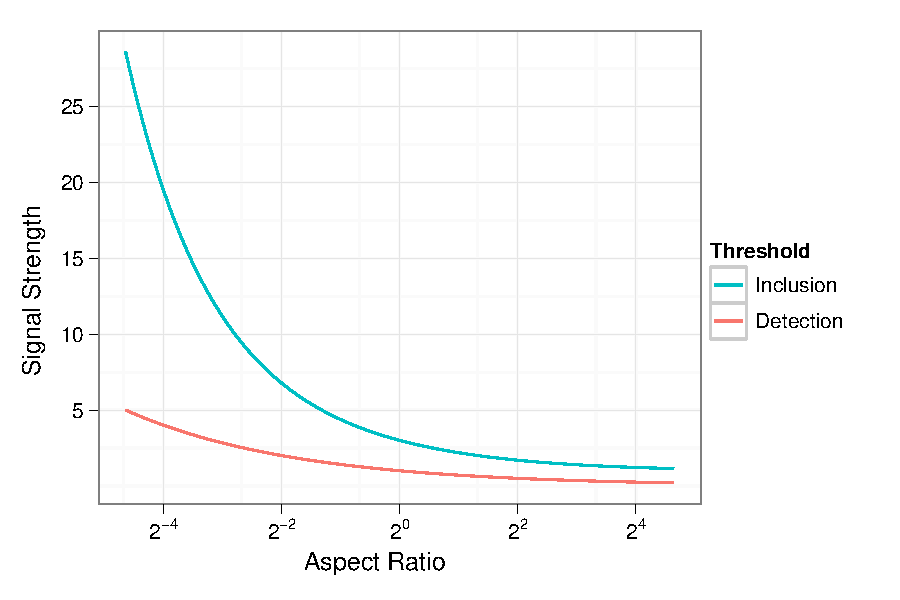
\includegraphics{frobenius-loss-cutoff}
    \caption{
        \captiontitle{Critical Signal Strength}
        Critical signal strength
        \(
            \frac{1 + \gamma^{-1}}{2}
            +
            \sqrt{
                \left( \frac{1 + \gamma^{-1} }{2} \right)^2
                +
                \frac{3}{\gamma}
            }
        \)
        plotted against the aspect ratio $\gamma = \frac{n}{p}$.  With
        respect to Frobenius loss, when the normalized signal strength 
        $\frac{\mu_i}{\sigma^2}$ is above this level it is beneficial to 
        include the $i$th term in the SVD approximation of 
        $\sqrt{n} \, \mU_n \mD_n \mV_n^\trans$.
    }\label{F:frobenius-loss-cutoff}
\end{figure}
